%!TEX root = ../egpaper_for_review.tex

\tikzstyle{nS}=[circle,minimum size = 0.6cm,inner sep = 0pt,draw, font=\small,align=left]
\tikzstyle{eS}=[thick,minimum size = 0.5cm,inner sep = 0pt,draw, font=\small,align=left]
\tikzstyle{eC}=[very thick,minimum size = 0.5cm,inner sep = 0pt,draw=red, font=\small,align=left]
\tikzstyle{eNC}=[very thick,minimum size = 0.5cm,inner sep = 0pt,draw=green, font=\small,align=left]
\tikzstyle{eNS}=[fill=white,minimum size = 0.5cm,inner sep = 0pt, font=\tiny,align=left]
\tikzstyle{eCC}=[very thick,dotted,minimum size = 0.5cm,inner sep = 0pt,draw=black, font=\small,align=left]

\begin{center}
\begin{figure}[h]
\begin{tiny}
\begin{subfigure}[t]{0.22\linewidth}
    \resizebox{\linewidth}{!}{
        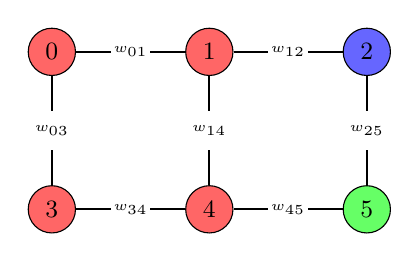
\begin{tikzpicture}[scale=1]%[x=1 cm, y=1 cm]
                \draw (2,2) node[nS,fill=red!60] (n0) {$0$}; 
                \draw (4,2) node[nS,fill=red!60] (n1) {$1$};
                \draw (6,2) node[nS,fill=blue!60] (n2) {$2$};
                \draw (2,0) node[nS,fill=red!60] (n3) {$3$}; 
                \draw (4,0) node[nS,fill=red!60] (n4) {$4$};
                \draw (6,0) node[nS,fill=green!60] (n5) {$5$};
                \path
                    (n0) edge[eS] node[eNS]{$w_{01}$} (n1) 
                    (n1) edge[eS] node[eNS]{$w_{12}$} (n2) 
                    (n3) edge[eS] node[eNS]{$w_{34}$} (n4) 
                    (n4) edge[eS] node[eNS]{$w_{45}$} (n5)
                    (n0) edge[eS] node[eNS]{$w_{03}$} (n3)
                    (n1) edge[eS] node[eNS]{$w_{14}$} (n4)
                    (n2) edge[eS] node[eNS]{$w_{25}$} (n5)
                ;
        \end{tikzpicture}
    }
\caption{ \tiny{node labels}}
\label{fig:not_a}
\end{subfigure}
\hfill
\begin{subfigure}[t]{0.22\linewidth}
    \resizebox{\linewidth}{!}{
        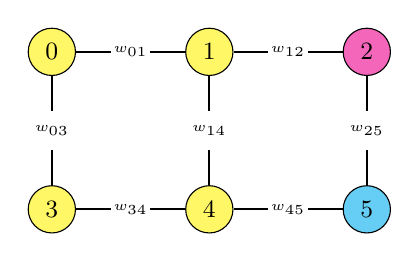
\begin{tikzpicture}[scale=1]%[x=1 cm, y=1 cm]
                \draw (2,2) node[nS,fill=yellow!60] (n0) {$0$}; 
                \draw (4,2) node[nS,fill=yellow!60] (n1) {$1$};
                \draw (6,2) node[nS,fill=magenta!60] (n2) {$2$};
                \draw (2,0) node[nS,fill=yellow!60] (n3) {$3$}; 
                \draw (4,0) node[nS,fill=yellow!60] (n4) {$4$};
                \draw (6,0) node[nS,fill=cyan!60] (n5) {$5$};
                \path
                    (n0) edge[eS] node[eNS]{$w_{01}$} (n1) 
                    (n1) edge[eS] node[eNS]{$w_{12}$} (n2) 
                    (n3) edge[eS] node[eNS]{$w_{34}$} (n4) 
                    (n4) edge[eS] node[eNS]{$w_{45}$} (n5)
                    (n0) edge[eS] node[eNS]{$w_{03}$} (n3)
                    (n1) edge[eS] node[eNS]{$w_{14}$} (n4)
                    (n2) edge[eS] node[eNS]{$w_{25}$} (n5)
                ;
        \end{tikzpicture}
    }
\caption{ \tiny{node labels}}
\label{fig:not_b}
\end{subfigure}
\hfill
\begin{subfigure}[t]{0.22\linewidth}
    \resizebox{\linewidth}{!}{
        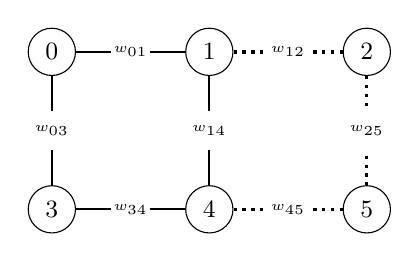
\begin{tikzpicture}[scale=1]%[x=1 cm, y=1 cm]
                \draw (2,2) node[nS] (n0) {$0$}; 
                \draw (4,2) node[nS] (n1) {$1$};
                \draw (6,2) node[nS] (n2) {$2$};
                \draw (2,0) node[nS] (n3) {$3$}; 
                \draw (4,0) node[nS] (n4) {$4$};
                \draw (6,0) node[nS] (n5) {$5$};
                \path
                    (n0) edge[eS] node[eNS]{$w_{01}$} (n1) 
                    (n1) edge[eCC] node[eNS]{$w_{12}$} (n2) 
                    (n3) edge[eS] node[eNS]{$w_{34}$} (n4) 
                    (n4) edge[eCC] node[eNS]{$w_{45}$} (n5)
                    (n0) edge[eS] node[eNS]{$w_{03}$} (n3)
                    (n1) edge[eS] node[eNS]{$w_{14}$} (n4)
                    (n2) edge[eCC] node[eNS]{$w_{25}$} (n5)
                ;
        \end{tikzpicture}
    }
\caption{ \tiny{edge labels}}
\label{fig:not_c}
\end{subfigure}
\hfill
\begin{subfigure}[t]{0.22\linewidth}
    \resizebox{\linewidth}{!}{
        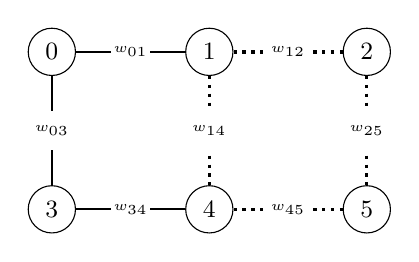
\begin{tikzpicture}[scale=1]%[x=1 cm, y=1 cm]
                \draw (2,2) node[nS] (n0) {$0$}; 
                \draw (4,2) node[nS] (n1) {$1$};
                \draw (6,2) node[nS] (n2) {$2$};
                \draw (2,0) node[nS] (n3) {$3$}; 
                \draw (4,0) node[nS] (n4) {$4$};
                \draw (6,0) node[nS] (n5) {$5$};
                \path
                    (n0) edge[eS] node[eNS]{$w_{01}$} (n1) 
                    (n1) edge[eCC] node[eNS]{$w_{12}$} (n2) 
                    (n3) edge[eS] node[eNS]{$w_{34}$} (n4) 
                    (n4) edge[eCC] node[eNS]{$w_{45}$} (n5)
                    (n0) edge[eS] node[eNS]{$w_{03}$} (n3)
                    (n1) edge[eCC] node[eNS]{$w_{14}$} (n4)
                    (n2) edge[eCC] node[eNS]{$w_{25}$} (n5)
                ;
        \end{tikzpicture}
    }
\caption{ \tiny{dangling edges}}
\label{fig:not_d}
\end{subfigure}
\end{tiny}
\caption{
Node labels suffers from ambiguities. 
The node labels in 
~\ref{fig:not_a} and ~\ref{fig:not_b} are 
different, but encode the same partition.
The edge labels in ~\ref{fig:not_c}
encodes the same partition. Edge
labels do not suffer from ambiguities, but only
edge labels without \emph{any dangling edges}
encode a valid partition. In ~\ref{fig:not_d}
there are dangling edges. Node $1$ and $4$ 
are in the same connected component, 
and at the same time $w_{14}$ wants to keep
them in separate connected components.
Therefore this does
not correspond to a valid partitioning.
}\label{fig:notation}
\end{figure}
\end{center}



